
\section{Results}
\label{sec:results}
Our results are displayed in Figure $1$.
\begin{figure}[htb]
  \centering % centers the entire table

  % The following line sets the parameters of the table: we'll have
  % three columns (one per 'c'), each
  % column will be centered (hence the 'c'; 'l' or 'r' will left or
  % right justify the column) and the columns
  % will have lines between them (that's the purpose of the |s between
  % the 'c's).
  \begin{tabular}{|c|c|c|} 
    \hline \hline % draws two horizontal lines at the top of the table
    \textbf{Model Settings} & \textbf{Moreover} & \textbf{OPoint} \\ % separate column contents using the &
    \hline % line after the column headers
    LinearSVR, L1 & $-0.059$ & $-0.034$ \\
    Linear SVR, L2 & $0.826$ & $0.860$\\
    RFR, max\_feature = 'None' & $0.125$ & $0.373$ \\
    RFR, max\_feature = 'sqrt' & $0.263$ & $0.350$ \\
    RFR, max\_feature = 'log2' & $0.096$ & $0.337$ \\
    Lasso regression & $0.554$ & $-0.435$ \\
    \hline \hline
  \end{tabular}

  % As with figures, *every* table should have a descriptive caption
  % and a label for ease of reference.
  \caption{Results under 10-folds Cross Validation}
  \label{tab:example}

\end{figure}
For \texttt{LinearSVR}, the r2 score improved substantially after we switched from L1 to L2 penalty. We think this is because the L2 penalty led to lower regularization strength. For the different C values we tested, $1.5$ turned out to be the one that gave us the best result among all. \\
For \texttt{RandomForestRegressor}, we started out using a smaller number of trees, ranging from $5$ to $25$ trees. However, our initial r2 scores from \texttt{RFR} yielded extremely high variance, ranging from $0.249$ to $-4.88$. We realized that this was correlated to the smaller number of trees we had, so we increased our tree size substantially. Our results can be seen from the figure above, and a number of $150$ and $200$ trees seemed to consistently generated the best results.\\
Overall, our models still had relatively high variance in results. Under the $10$-folds cross validation we performed for \texttt{RFR} and \texttt{LinearSVR} for example, we saw that the r2 scores could still range from as low as $-0.257$ to as high as $0.989$. Figure $2$ below visualizes one example of such variance. We thought this was because we had way too many features to deal with in this project, and this substantially increased the randomness of the results. For both \texttt{RandomForestRegressor} and \texttt{LinearSVR}, the results are also low-biased. We assumed the high variance, low bias combination happened because there were too many decision nodes to go through before each model could arrive at a result. Because of this, even a small change in input variable could result in completely different regression models, hence leading to the phenomenon that we observed.\\
\begin{figure}[htb]

  \centering  % centers the image in the column

  % replace the second argument below with your filename. I like to
  % place all my figures in a sub-directory to keep things organized
  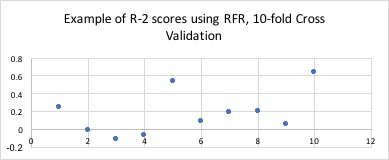
\includegraphics[width=0.47\textwidth]{1.jpg}

  % *Every* figure should have a descriptive caption.
  \caption{Results of R-2 scores derived from the RFR model, using n\_estimator = $100$, max\_feature = 'sqrt' and max\_depth = $20$. }

  % The label is a handle you create so that you can refer to this
  % figure (using the \ref{} command) from other parts of your
  % document. LaTeX automatically renumbers figures and updates
  % references when you recompile, so you should do it this way rather
  % than hard-coding in references. Notice that I've also been
  % creating labels for the various sections in the document; I could
  % use \ref{} command to refer to those sections using their labels
  % too.
  \label{fig:tex}
\end{figure}

The overall performance of the Lasso regression on our dataset was fairly good for articles from Moreover, but not as satisfactory for articles from Opoint. The scores obtained after a 10-fold cross validation and hyper-parameter tuning on alpha did not lead to remarkable improvement. In general, we expected that hyper-parameter tuning on alpha would enhance the performance of the model, since using smaller alpha values reduces the amount of penalization \cite{AnalyticsVidhya}; however, the results obtained after cross validation proved that \textttt{Lasso} performed better than \texttt{RFR} on the Moreover articles, and it performed significantly worse on the articles from Opoint. 

As mentioned in the previous sections, later on in our project we realized that without deleting duplicates in our data frame, we were essentially overestimating our model performance, since we were testing the model on what it was trained on. The results we delivered in Figure $1$ were recorded after we had deleted the duplicates. We compared the two sets of results before and after we discarded duplicates, and the results are shown in Figure $3$. Interestingly, \texttt{RFR} was affected a lot more than \texttt{LinearSVR} was, perhaps due to the fact that \texttt{LinearSVR} is well-performed for text analytics problem to begin with. However, keeping duplicates simply would create excessive optimism for \texttt{RFR}'s model performances. 
\begin{figure}[htb]

  \centering  % centers the image in the column

  % replace the second argument below with your filename. I like to
  % place all my figures in a sub-directory to keep things organized
  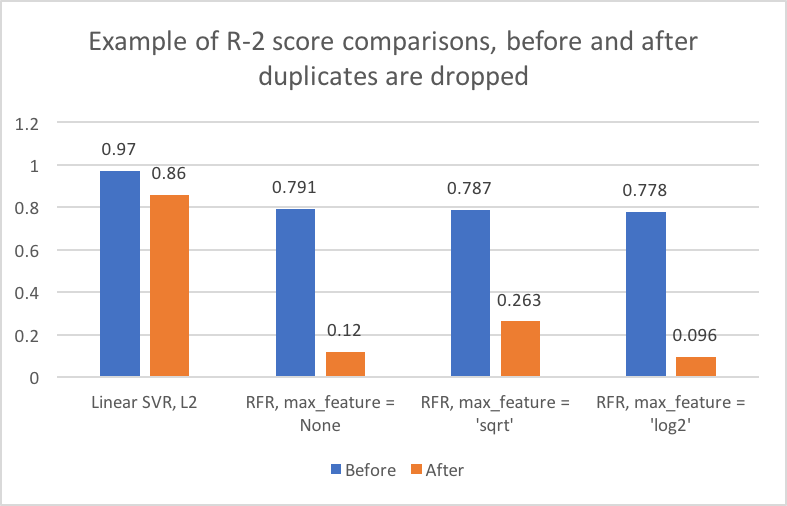
\includegraphics[width=0.47\textwidth]{2.png}
 \caption{Visualization of the effects after duplicates were dropped}
  % *Every* figure should have a descriptive caption.
  % The label is a handle you create so that you can refer to this
  % figure (using the \ref{} command) from other parts of your
  % document. LaTeX automatically renumbers figures and updates
  % references when you recompile, so you should do it this way rather
  % than hard-coding in references. Notice that I've also been
  % creating labels for the various sections in the document; I could
  % use \ref{} command to refer to those sections using their labels
  % too.
  \label{fig:tex}

\end{figure}




